\documentclass{article}\usepackage[]{graphicx}\usepackage[]{color}
%% maxwidth is the original width if it is less than linewidth
%% otherwise use linewidth (to make sure the graphics do not exceed the margin)
\makeatletter
\def\maxwidth{ %
  \ifdim\Gin@nat@width>\linewidth
    \linewidth
  \else
    \Gin@nat@width
  \fi
}
\makeatother

\definecolor{fgcolor}{rgb}{0.345, 0.345, 0.345}
\newcommand{\hlnum}[1]{\textcolor[rgb]{0.686,0.059,0.569}{#1}}%
\newcommand{\hlstr}[1]{\textcolor[rgb]{0.192,0.494,0.8}{#1}}%
\newcommand{\hlcom}[1]{\textcolor[rgb]{0.678,0.584,0.686}{\textit{#1}}}%
\newcommand{\hlopt}[1]{\textcolor[rgb]{0,0,0}{#1}}%
\newcommand{\hlstd}[1]{\textcolor[rgb]{0.345,0.345,0.345}{#1}}%
\newcommand{\hlkwa}[1]{\textcolor[rgb]{0.161,0.373,0.58}{\textbf{#1}}}%
\newcommand{\hlkwb}[1]{\textcolor[rgb]{0.69,0.353,0.396}{#1}}%
\newcommand{\hlkwc}[1]{\textcolor[rgb]{0.333,0.667,0.333}{#1}}%
\newcommand{\hlkwd}[1]{\textcolor[rgb]{0.737,0.353,0.396}{\textbf{#1}}}%
\let\hlipl\hlkwb

\usepackage{framed}
\makeatletter
\newenvironment{kframe}{%
 \def\at@end@of@kframe{}%
 \ifinner\ifhmode%
  \def\at@end@of@kframe{\end{minipage}}%
  \begin{minipage}{\columnwidth}%
 \fi\fi%
 \def\FrameCommand##1{\hskip\@totalleftmargin \hskip-\fboxsep
 \colorbox{shadecolor}{##1}\hskip-\fboxsep
     % There is no \\@totalrightmargin, so:
     \hskip-\linewidth \hskip-\@totalleftmargin \hskip\columnwidth}%
 \MakeFramed {\advance\hsize-\width
   \@totalleftmargin\z@ \linewidth\hsize
   \@setminipage}}%
 {\par\unskip\endMakeFramed%
 \at@end@of@kframe}
\makeatother

\definecolor{shadecolor}{rgb}{.97, .97, .97}
\definecolor{messagecolor}{rgb}{0, 0, 0}
\definecolor{warningcolor}{rgb}{1, 0, 1}
\definecolor{errorcolor}{rgb}{1, 0, 0}
\newenvironment{knitrout}{}{} % an empty environment to be redefined in TeX

\usepackage{alltt}
\usepackage{multirow}
\usepackage{multicol}
\usepackage{graphicx}
\usepackage{hyperref}
\hypersetup{%
  colorlinks = true,
  linkcolor  = black
}

\title{Evaluating Monthly Trends using CHCN-Daily}
\author{Marc Los Huertos}

% Setting up the margins, etc for R




\IfFileExists{upquote.sty}{\usepackage{upquote}}{}
\begin{document}

\maketitle
\tableofcontents

\begin{abstract}
\noindent This SOP will provide the tools to analyze the CDO climate data for long-term trends in the daily data. We will also create monthly averages and determine if some months have a stronger trend than others.   

\end{abstract}


\section{Introduction}

\subsection{Goals for This Document}

This document provides EA students with the methods to analyze climate data based on monthly averages and evaluate if these data are reliable compared to the CHCN-Monthly and investigate sources of uncertainty. 

\subsection{To Begin}

You should have R code that generates a plot of daily TMAX data for a site with a best fit line overlaid. If not, please go back to SOP85.


\subsection{Generalized Steps}

In this SOP you will ...

\begin{enumerate}
  \item create new variables for date and month;
  \item create a new dataframe with monthly averages;
  \item model and estimate average trend for each month;
  \item evaluate the validity of the models; and
  \item interpret the trend data
\end{enumerate}


\subsection{Regression and Climate Change}

One of the ourcomes of the linear regression is to estimate the best fit line

\begin{equation}
y = mx + b + \epsilon,
\end{equation}

where $\epsilon$ is an estimate of the error. In addition, two other estimates are provided, one for the slope, $m$, and the y-intercept, $b$. 

But these estimates are also hypotheses, where the null hypothesis is:

\begin{description}
  \item[slope is zero] Rejecting the null hypothesis would be support the alternative hypothesis, or the estimate of the slope. 
  \item[y-intercept is zero] Rejecting the null hypothesis would support the alternative hypothesis, the estimate of the y-intercept.
\end{description}

Okay, let's see if we can do this for our Bangkok data. Let's test if there is a significant change of daily maximum temperatures (TMAX) with time. Thus, in general terms, Maximum temperature is a function of time, or $TMAX = f(Time)$. 

\begin{equation}
TMAX \sim \alpha + \beta * time + \epsilon
\end{equation}

Translating this in R will take some additional tricks besides just getting the code figured out. First, we need to identify the predictor variable, 'NewDate', in the data frame which we created in SOP85. 

Because these data are in a time series, they are serially correlated, meaning that the June sample will be more like the July sample than the August sample. In addition, the June 2010 sample will be similar to the June 2009 sample. These correlation violate the assumption of independence, but for now, we will ignore this violation and just create a linear model in bliss. 

For the response variable, we will use the daily maximum temeratures, TMAX. Remember there are some missing data, it will be interesting to note how R deals with that.

First, let's create a plot of data using \texttt{plot()}, whose format is \texttt{plot(x, y)} or \texttt{plot(y ~ x)}. We will use the later for now, 

\begin{figure}
\label{fig:test12}
\caption{Maximum daily temperatures for Bangkok, Thailand.}
\begin{knitrout}
\definecolor{shadecolor}{rgb}{0.969, 0.969, 0.969}\color{fgcolor}
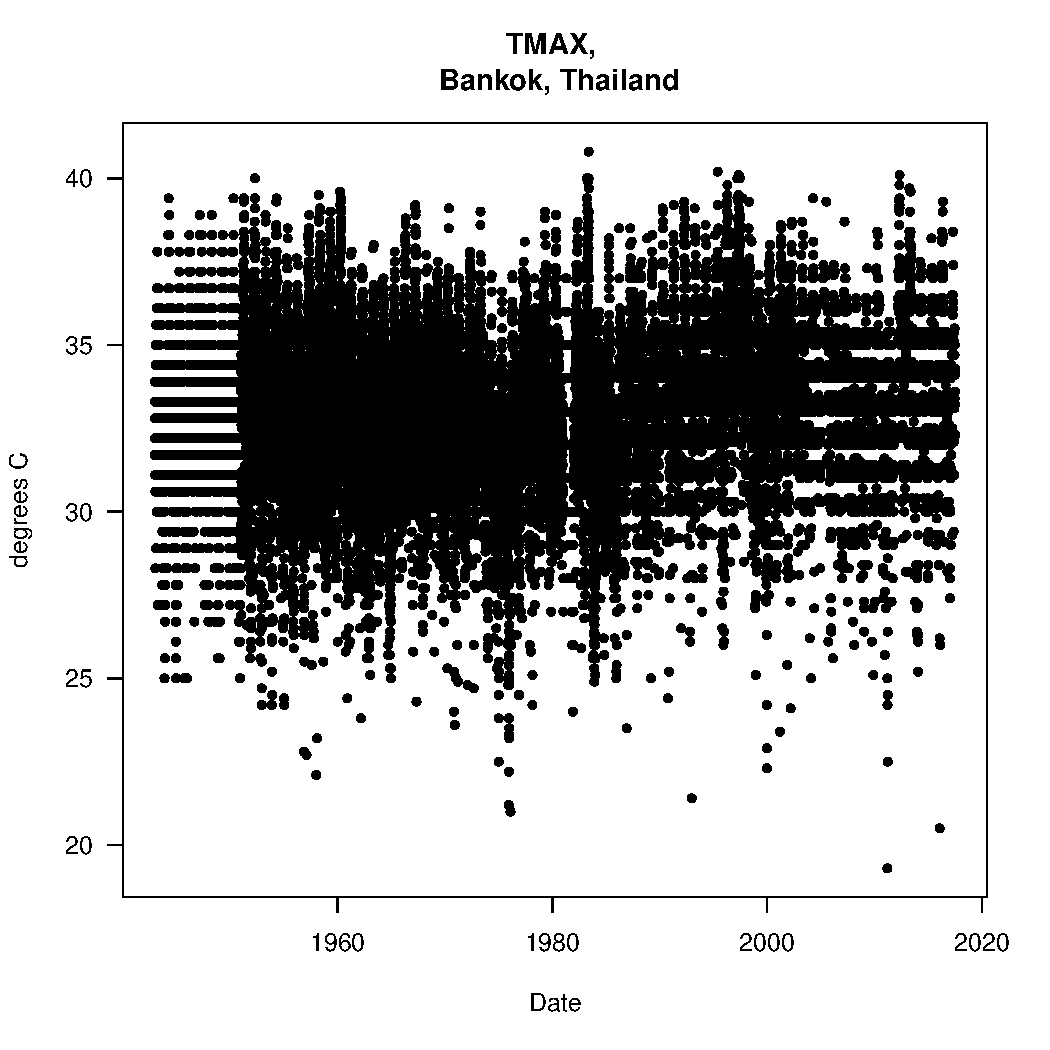
\includegraphics[width=\maxwidth]{figure/Tmaxplot-1} 

\end{knitrout}
\end{figure}

We use the \texttt{lm()} function that arrange the results in-line with a regression model. This syntax is straight forward,  

\begin{knitrout}
\definecolor{shadecolor}{rgb}{0.969, 0.969, 0.969}\color{fgcolor}\begin{kframe}
\begin{alltt}
\hlkwd{lm}\hlstd{(TMAX} \hlopt{~} \hlstd{NewDate,} \hlkwc{data}\hlstd{=climate_data)}
\end{alltt}
\begin{verbatim}
## 
## Call:
## lm(formula = TMAX ~ NewDate, data = climate_data)
## 
## Coefficients:
## (Intercept)      NewDate  
##   3.289e+01    2.702e-05
\end{verbatim}
\end{kframe}
\end{knitrout}

From this model, we learn that the change in $TMAX$ is 
0 degrees $year^{-1}$. Figure~\ref{fig:TMAX_trend} shows a trend of increasing maximum temperatures.

% Additional LaTeX code to add caption to figure
\begin{figure}
\label{fig:TMAX_trend}
\caption{Maximum Daily Temperatures in Bangkok, Thailand.}
\begin{knitrout}
\definecolor{shadecolor}{rgb}{0.969, 0.969, 0.969}\color{fgcolor}
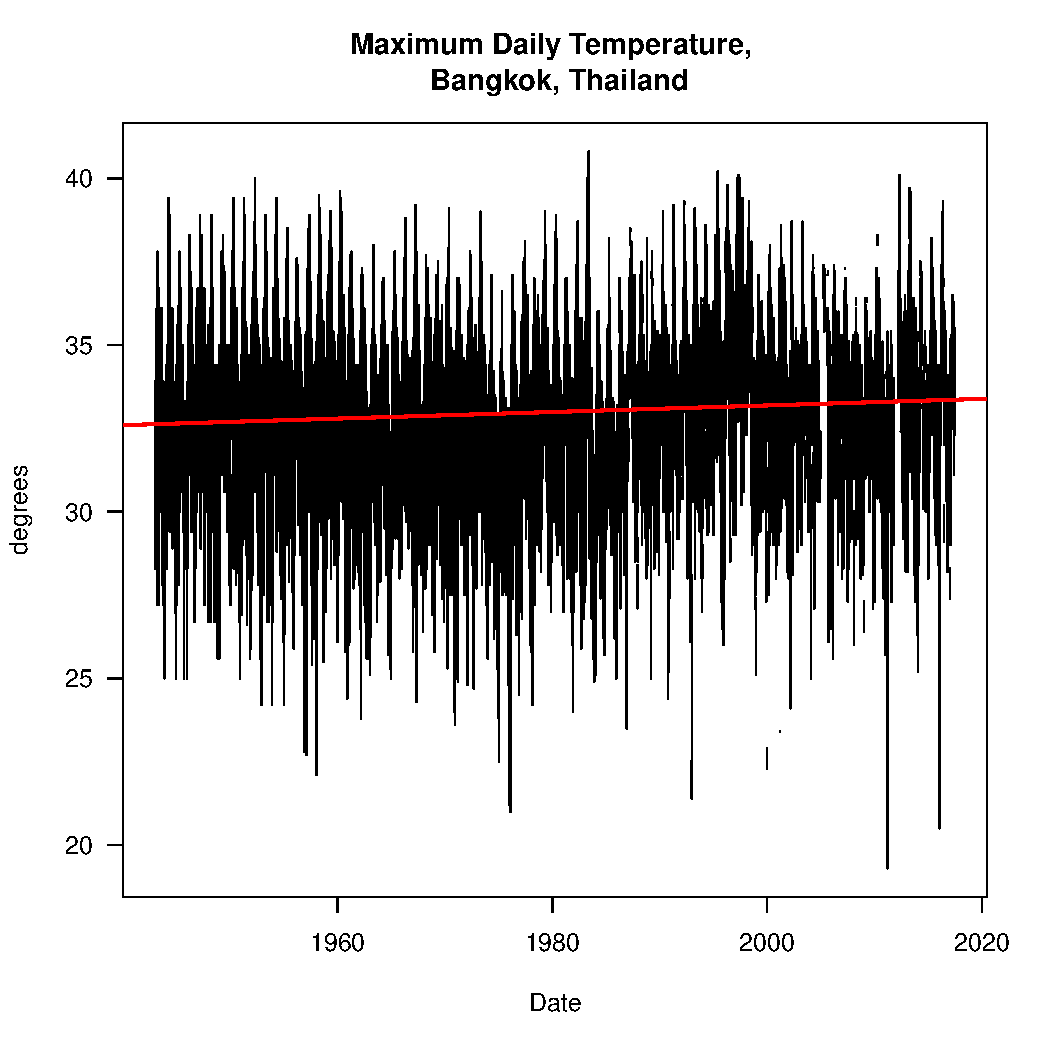
\includegraphics[width=\maxwidth]{figure/unnamed-chunk-3-1} 

\end{knitrout}
\end{figure}

Now determine test the null hypotheses and use the \texttt{summary()} function to display many of the important regression results.

\begin{knitrout}
\definecolor{shadecolor}{rgb}{0.969, 0.969, 0.969}\color{fgcolor}\begin{kframe}
\begin{alltt}
\hlkwd{summary}\hlstd{(}\hlkwd{lm}\hlstd{(TMAX} \hlopt{~} \hlstd{NewDate,} \hlkwc{data}\hlstd{=climate_data))}
\end{alltt}
\begin{verbatim}
## 
## Call:
## lm(formula = TMAX ~ NewDate, data = climate_data)
## 
## Residuals:
##      Min       1Q   Median       3Q      Max 
## -13.9974  -1.3193   0.0782   1.4717   7.7771 
## 
## Coefficients:
##              Estimate Std. Error t value Pr(>|t|)
## (Intercept) 3.289e+01  1.631e-02 2016.35   <2e-16
## NewDate     2.702e-05  2.140e-06   12.62   <2e-16
##                
## (Intercept) ***
## NewDate     ***
## ---
## Signif. codes:  
## 0 '***' 0.001 '**' 0.01 '*' 0.05 '.' 0.1 ' ' 1
## 
## Residual standard error: 2.329 on 21958 degrees of freedom
##   (5066 observations deleted due to missingness)
## Multiple R-squared:  0.007202,	Adjusted R-squared:  0.007157 
## F-statistic: 159.3 on 1 and 21958 DF,  p-value: < 2.2e-16
\end{verbatim}
\end{kframe}
\end{knitrout}

Based on the results, we reject the null hypotheses, i.e. the events that this might occur by chance is small: 2x10$^{-16}$ for the slope is zero and p < 2x10$^{-16}$ for the y-intercept is zero. 

In addition, we have some information on the residuals, and $R^2$ estimates, which are important to interpret the model. 

For now, we can appreciate the the temperature is changing, i.e. increasing, with a slope of 2.7x10$^{-5}$ degrees C per year. 

\subsubsection{Creating Monthly Averages of Daily Maximum Temperatures}

One of the first things to note is how messy the data look and there are lots of sources of variation. For example, we expect months to respond differently to the climate change. To assess this, we will now analyze the data for monthly means of the maximum temperatures.

\subsubsection{Creating Monthly Means}

To create monthly means, we need to disagragate the NewDate variable into a month and year variables.

First we can use the \texttt{as.Date()} function to extract a portion of the date, where \%m is for month and \%Y is for a four digit year. Then, we create new variables in our dataframe, one for month and one for year.

\begin{knitrout}
\definecolor{shadecolor}{rgb}{0.969, 0.969, 0.969}\color{fgcolor}\begin{kframe}
\begin{alltt}
\hlstd{climate_data}\hlopt{$}\hlstd{Month} \hlkwb{=} \hlkwd{format}\hlstd{(}\hlkwd{as.Date}\hlstd{(climate_data}\hlopt{$}\hlstd{NewDate),} \hlkwc{format} \hlstd{=} \hlstr{"%m"}\hlstd{)}
\hlstd{climate_data}\hlopt{$}\hlstd{Year} \hlkwb{=} \hlkwd{format}\hlstd{(climate_data}\hlopt{$}\hlstd{NewDate,} \hlkwc{format}\hlstd{=}\hlstr{"%Y"}\hlstd{)}
\end{alltt}
\end{kframe}
\end{knitrout}

After creating the month and year as separate variables, we can use them to caculate the mean using the \texttt{aggregate()} function. In the code below, we can also calculate the standard deviation too, although I haven't used this measure in this document, several students have asked for this for their analysis.

\begin{knitrout}
\definecolor{shadecolor}{rgb}{0.969, 0.969, 0.969}\color{fgcolor}\begin{kframe}
\begin{alltt}
\hlstd{MonthlyTMAXMean} \hlkwb{=} \hlkwd{aggregate}\hlstd{(TMAX} \hlopt{~} \hlstd{Month} \hlopt{+} \hlstd{Year, climate_data, mean)}

\hlstd{MonthlyTMAXMean}\hlopt{$}\hlstd{YEAR} \hlkwb{=} \hlkwd{as.numeric}\hlstd{(MonthlyTMAXMean}\hlopt{$}\hlstd{Year)}
\hlstd{MonthlyTMAXMean}\hlopt{$}\hlstd{MONTH} \hlkwb{=} \hlkwd{as.numeric}\hlstd{(MonthlyTMAXMean}\hlopt{$}\hlstd{Month)}
\end{alltt}
\end{kframe}
\end{knitrout}

\begin{knitrout}
\definecolor{shadecolor}{rgb}{0.969, 0.969, 0.969}\color{fgcolor}\begin{kframe}
\begin{alltt}
\hlkwd{str}\hlstd{(MonthlyTMAXMean)}
\end{alltt}
\begin{verbatim}
## 'data.frame':	888 obs. of  5 variables:
##  $ Month: chr  "01" "02" "03" "04" ...
##  $ Year : chr  "1943" "1943" "1943" "1943" ...
##  $ TMAX : num  32.2 33.2 34.9 33.5 33.8 ...
##  $ YEAR : num  1943 1943 1943 1943 1943 ...
##  $ MONTH: num  1 2 3 4 5 6 7 8 9 10 ...
\end{verbatim}
\end{kframe}
\end{knitrout}


\begin{knitrout}
\definecolor{shadecolor}{rgb}{0.969, 0.969, 0.969}\color{fgcolor}\begin{kframe}
\begin{alltt}
\hlkwd{plot}\hlstd{(MonthlyTMAXMean}\hlopt{$}\hlstd{TMAX,} \hlkwc{ty}\hlstd{=}\hlstr{'l'}\hlstd{)}
\end{alltt}
\end{kframe}
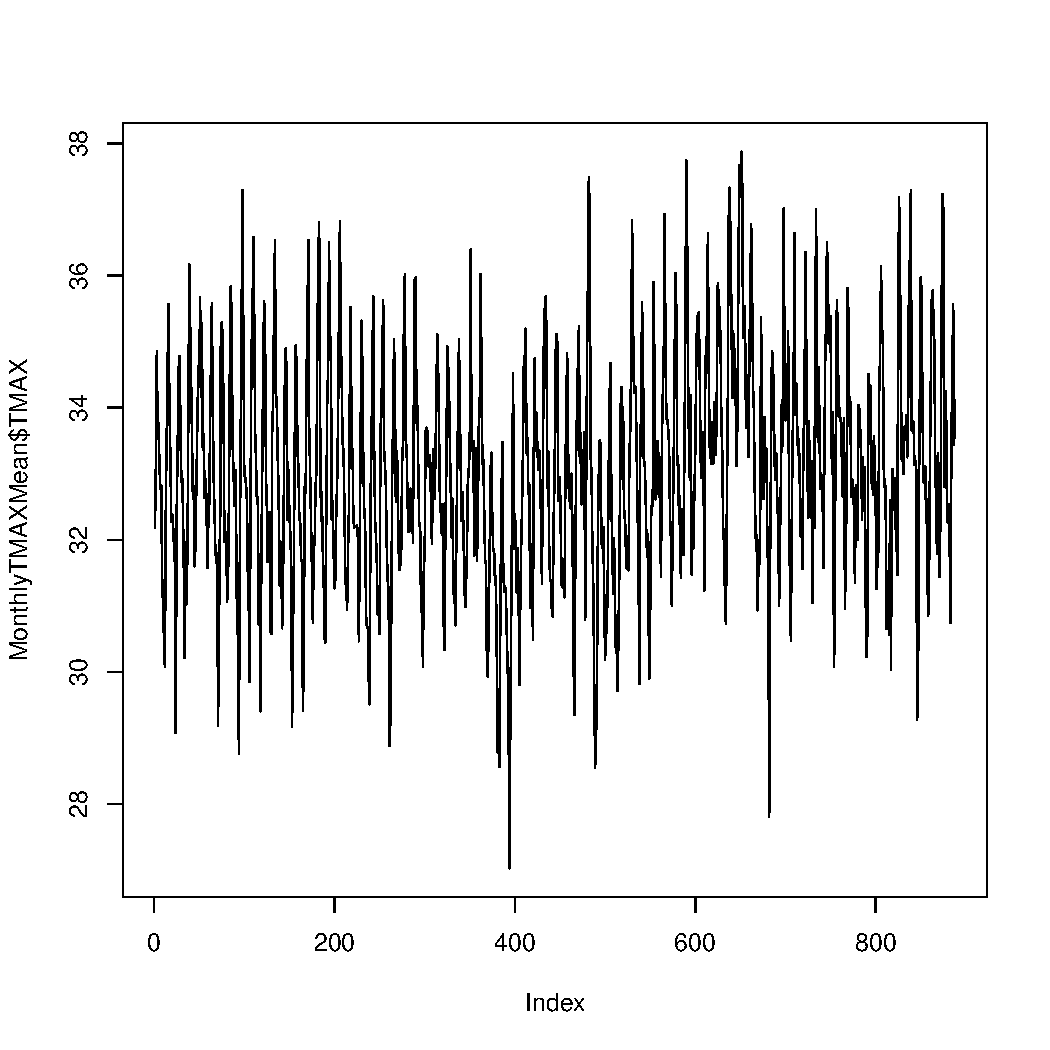
\includegraphics[width=\maxwidth]{figure/unnamed-chunk-4-1} 

\end{knitrout}


\subsection{Selecting for 1 Month -- May}

Perhaps, we can get a better handle on this stuff if we analyze for just one month at a time -- certainly easier to visualize!

\begin{knitrout}
\definecolor{shadecolor}{rgb}{0.969, 0.969, 0.969}\color{fgcolor}\begin{kframe}
\begin{alltt}
\hlcom{#plot(MonthlyTMAXMean$TMAX[MonthlyTMAXMean$Month=="05"], ty='l')}
\hlkwd{plot}\hlstd{(TMAX}\hlopt{~}\hlstd{YEAR,} \hlkwc{data}\hlstd{=MonthlyTMAXMean[MonthlyTMAXMean}\hlopt{$}\hlstd{Month}\hlopt{==}\hlstr{"05"}\hlstd{,],}
     \hlkwc{ty}\hlstd{=}\hlstr{'l'}\hlstd{,} \hlkwc{xlim}\hlstd{=}\hlkwd{c}\hlstd{(}\hlnum{1950}\hlstd{,} \hlnum{2020}\hlstd{))}
\hlstd{May.lm} \hlkwb{<-} \hlkwd{lm}\hlstd{(TMAX}\hlopt{~}\hlstd{YEAR,} \hlkwc{data}\hlstd{=MonthlyTMAXMean[MonthlyTMAXMean}\hlopt{$}\hlstd{Month}\hlopt{==}\hlstr{"05"}\hlstd{,])}
\hlkwd{summary}\hlstd{(May.lm)}
\end{alltt}
\begin{verbatim}
## 
## Call:
## lm(formula = TMAX ~ YEAR, data = MonthlyTMAXMean[MonthlyTMAXMean$Month == 
##     "05", ])
## 
## Residuals:
##      Min       1Q   Median       3Q      Max 
## -2.85376 -0.93210 -0.04633  0.81231  3.15347 
## 
## Coefficients:
##              Estimate Std. Error t value Pr(>|t|)
## (Intercept) 17.238621  13.753642   1.253    0.214
## YEAR         0.008756   0.006946   1.261    0.211
## 
## Residual standard error: 1.302 on 73 degrees of freedom
## Multiple R-squared:  0.0213,	Adjusted R-squared:  0.007897 
## F-statistic: 1.589 on 1 and 73 DF,  p-value: 0.2115
\end{verbatim}
\begin{alltt}
\hlkwd{abline}\hlstd{(}\hlkwd{coef}\hlstd{(May.lm),} \hlkwc{col}\hlstd{=}\hlstr{"red"}\hlstd{)}
\end{alltt}
\end{kframe}
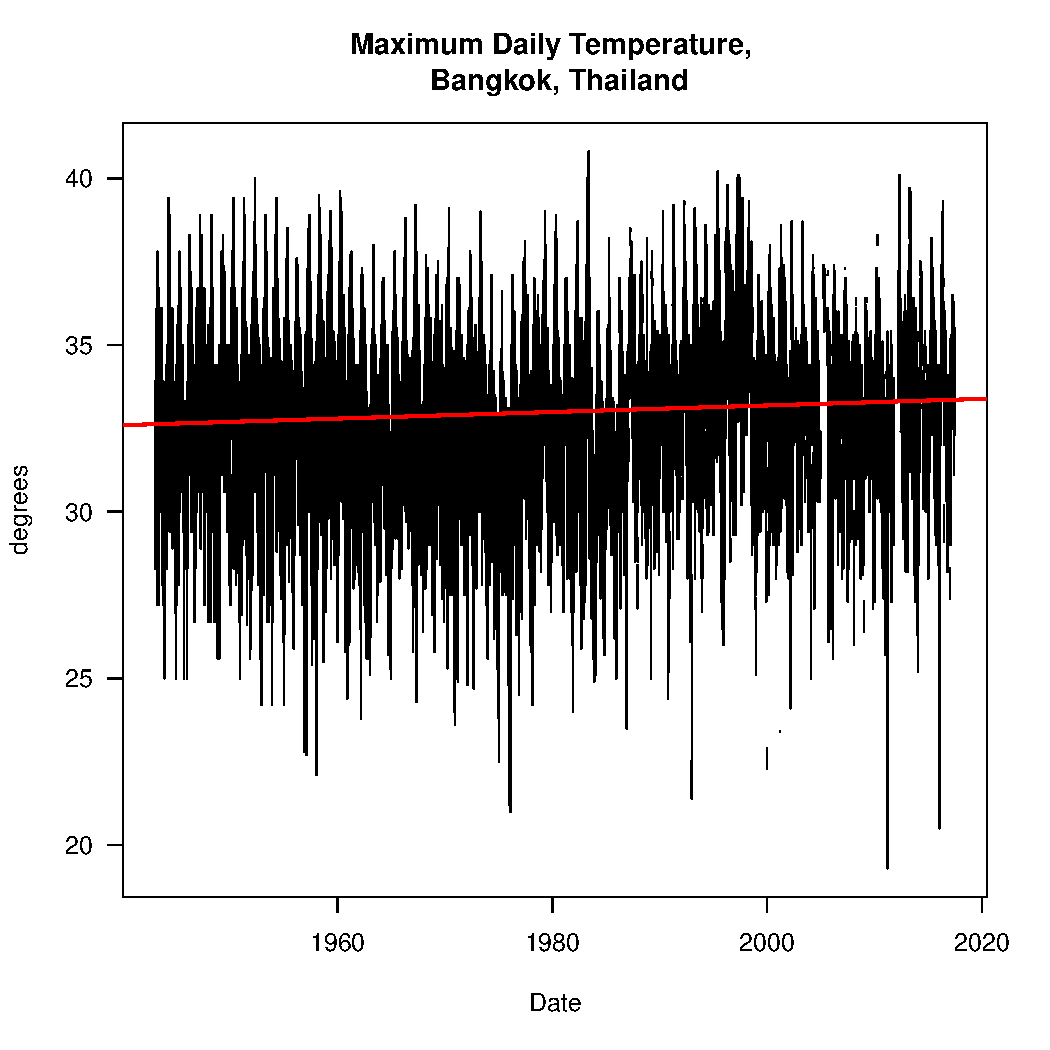
\includegraphics[width=\maxwidth]{figure/unnamed-chunk-5-1} 

\end{knitrout}

Now, the change is 0.0088 degress C/year or 0.876 degress C/100 years with a probability of 0.2115. Although we can't reject the null hypothesis, we find the method to be fairly straightforward! 

%https://feliperego.github.io/blog/2015/10/23/Interpreting-Model-Output-In-R

\subsection{Testing all the Months}

I think you should evaluate every month and see what happens. You might also consider looking at the TMIN as well. Could be important!\footnote{What about multiple hypotheses in one dataset!}

Below, I have create code to evaluate all of the months at once, but you may prefer to go through each month manually and change the number from 5 to other months of the year. 

\begin{figure}
\begin{knitrout}
\definecolor{shadecolor}{rgb}{0.969, 0.969, 0.969}\color{fgcolor}\begin{kframe}
\begin{alltt}
\hlcom{# First I create a vector of months}
\hlstd{Months} \hlkwb{=} \hlkwd{c}\hlstd{(}\hlstr{"January"}\hlstd{,} \hlstr{"February"}\hlstd{,} \hlstr{"March"}\hlstd{,} \hlstr{"April"}\hlstd{,}
    \hlstr{"May"}\hlstd{,} \hlstr{"June"}\hlstd{,} \hlstr{"July"}\hlstd{,} \hlstr{"August"}\hlstd{,} \hlstr{"September"}\hlstd{,} \hlstr{"October"}\hlstd{,}
    \hlstr{"November"}\hlstd{,} \hlstr{"December"}\hlstd{)}

\hlcom{# Create a panel so I can see all the figures at}
\hlcom{# once.}
\hlkwd{par}\hlstd{(}\hlkwc{mfrow} \hlstd{=} \hlkwd{c}\hlstd{(}\hlnum{4}\hlstd{,} \hlnum{3}\hlstd{),} \hlkwc{mar} \hlstd{=} \hlkwd{c}\hlstd{(}\hlnum{5}\hlstd{,} \hlnum{4}\hlstd{,} \hlnum{3}\hlstd{,} \hlnum{2}\hlstd{)} \hlopt{+} \hlnum{0.1}\hlstd{)}
\hlstd{TMAXresult} \hlkwb{<-} \hlnum{NA}
\hlkwa{for} \hlstd{(i} \hlkwa{in} \hlnum{1}\hlopt{:}\hlnum{12}\hlstd{) \{}
    \hlcom{# plot(MonthlyTMAXMean$TMAX[MonthlyTMAXMean$Month==i],}
    \hlcom{# ty='l')}
    \hlkwd{plot}\hlstd{(TMAX} \hlopt{~} \hlstd{YEAR,} \hlkwc{data} \hlstd{= MonthlyTMAXMean[MonthlyTMAXMean}\hlopt{$}\hlstd{MONTH} \hlopt{==}
        \hlstd{i, ],} \hlkwc{ty} \hlstd{=} \hlstr{"l"}\hlstd{,} \hlkwc{las} \hlstd{=} \hlnum{1}\hlstd{,} \hlkwc{xlim} \hlstd{=} \hlkwd{c}\hlstd{(}\hlnum{1940}\hlstd{,} \hlnum{2020}\hlstd{),}
        \hlkwc{main} \hlstd{= Months[i])}
    \hlstd{Month.lm} \hlkwb{<-} \hlkwd{lm}\hlstd{(TMAX} \hlopt{~} \hlstd{YEAR,} \hlkwc{data} \hlstd{= MonthlyTMAXMean[MonthlyTMAXMean}\hlopt{$}\hlstd{MONTH} \hlopt{==}
        \hlstd{i, ])}
    \hlkwd{summary}\hlstd{(Month.lm)}

    \hlkwd{abline}\hlstd{(}\hlkwd{coef}\hlstd{(Month.lm),} \hlkwc{col} \hlstd{=} \hlstr{"red"}\hlstd{)}

    \hlstd{TMAXresult} \hlkwb{<-} \hlkwd{rbind}\hlstd{(TMAXresult,} \hlkwd{cbind}\hlstd{(Months[i],}
        \hlkwd{round}\hlstd{(}\hlkwd{coef}\hlstd{(Month.lm)[}\hlnum{2}\hlstd{],} \hlnum{4}\hlstd{),} \hlkwd{round}\hlstd{(}\hlkwd{summary}\hlstd{(Month.lm)}\hlopt{$}\hlstd{coefficients[}\hlnum{2}\hlstd{,}
            \hlnum{4}\hlstd{],} \hlnum{4}\hlstd{),} \hlkwd{round}\hlstd{(}\hlkwd{summary}\hlstd{(Month.lm)}\hlopt{$}\hlstd{r.squared,}
            \hlnum{3}\hlstd{)))}
\hlstd{\}}
\end{alltt}
\end{kframe}
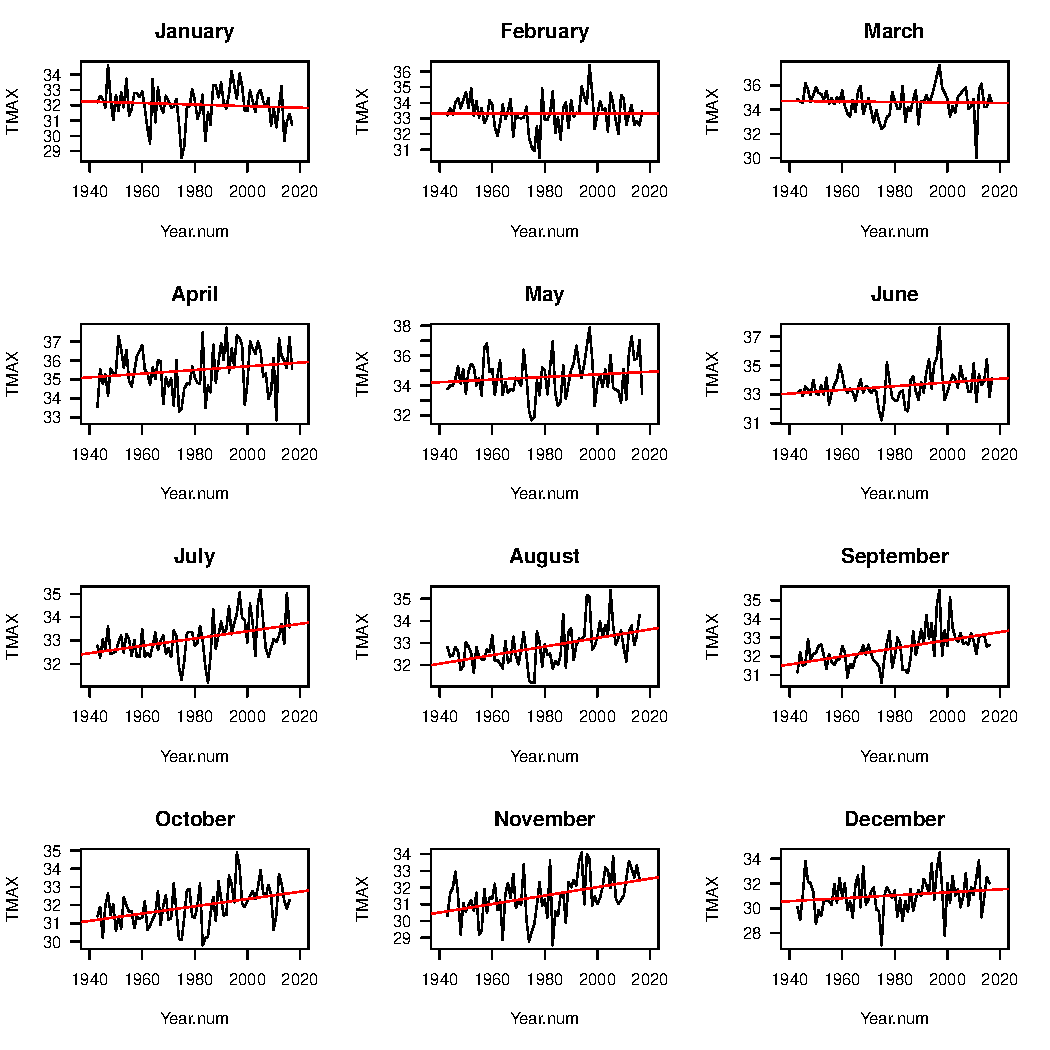
\includegraphics[width=\maxwidth]{figure/12MonthsTMAX-1} 

\end{knitrout}
\end{figure}

\subsection{Next Steps}

\subsubsection{Analyzing Minimum Daily Temperatures}

Alternatively, it might be important to evaluate changes to the daily mininum temperatures. Following the same steps we used before but using the TMIN instead of TMAX, let's analyze the monthly average of daily minimum temperatures by following these steps: 

\begin{enumerate}

\item First, let's plot the daily minimum temperatures, and as with the daily maximum temperatures, find tons of scatter (Table \ref{fig:TMIN_trend}).

% Additional LaTeX code to add caption to figure
\begin{figure}
\label{fig:TMIN_trend}
\caption{Minimum Daily Temperatures in Bangkok, Thailand.}
\begin{knitrout}
\definecolor{shadecolor}{rgb}{0.969, 0.969, 0.969}\color{fgcolor}
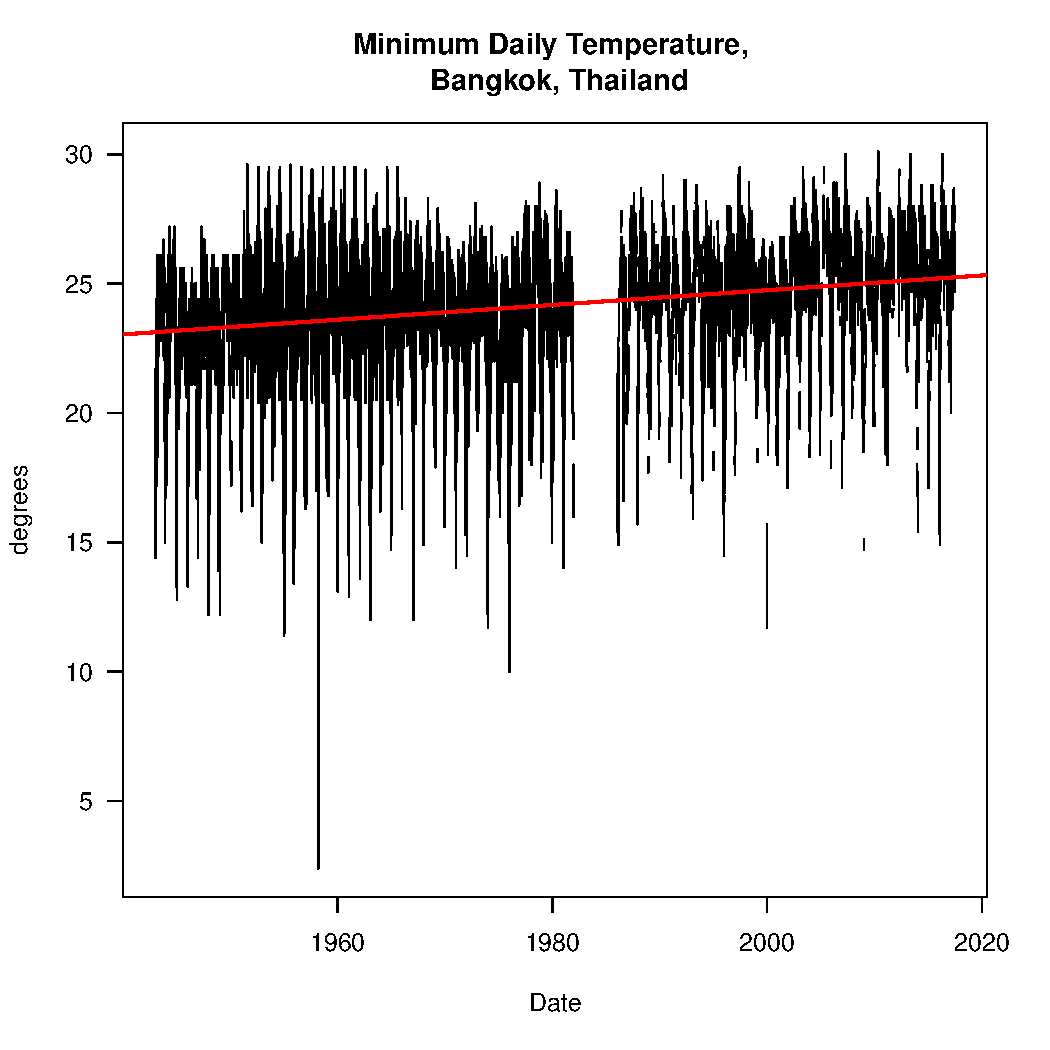
\includegraphics[width=\maxwidth]{figure/unnamed-chunk-6-1} 

\end{knitrout}
\end{figure}

There appears to be a trend, but it's clouded with lots of variation. 

  \item We create a monthly TMIN mean for each month.

\begin{knitrout}
\definecolor{shadecolor}{rgb}{0.969, 0.969, 0.969}\color{fgcolor}\begin{kframe}
\begin{alltt}
\hlstd{MonthlyTMINMean} \hlkwb{=} \hlkwd{aggregate}\hlstd{(TMIN} \hlopt{~} \hlstd{Month} \hlopt{+} \hlstd{Year, climate_data, mean)}

\hlstd{MonthlyTMINMean}\hlopt{$}\hlstd{YEAR} \hlkwb{=} \hlkwd{as.numeric}\hlstd{(MonthlyTMINMean}\hlopt{$}\hlstd{Year)}

\hlcom{# Fixing the Format of Month and Year as numeric}
\hlstd{MonthlyTMINMean}\hlopt{$}\hlstd{YEAR} \hlkwb{=} \hlkwd{as.numeric}\hlstd{(MonthlyTMINMean}\hlopt{$}\hlstd{Year)}
\hlstd{MonthlyTMINMean}\hlopt{$}\hlstd{MONTH} \hlkwb{=} \hlkwd{as.numeric}\hlstd{(MonthlyTMINMean}\hlopt{$}\hlstd{Month)}
\hlkwd{head}\hlstd{(MonthlyTMINMean)}
\end{alltt}
\begin{verbatim}
##   Month Year     TMIN YEAR MONTH
## 1    01 1943 18.54828 1943     1
## 2    02 1943 20.73077 1943     2
## 3    03 1943 23.39655 1943     3
## 4    04 1943 23.79259 1943     4
## 5    05 1943 24.87692 1943     5
## 6    06 1943 24.76429 1943     6
\end{verbatim}
\end{kframe}
\end{knitrout}

\item Create a plot of the monthly average of the daily minimum temperatures. 


\begin{knitrout}
\definecolor{shadecolor}{rgb}{0.969, 0.969, 0.969}\color{fgcolor}\begin{kframe}
\begin{alltt}
\hlkwd{plot}\hlstd{(MonthlyTMINMean}\hlopt{$}\hlstd{TMIN,} \hlkwc{ty}\hlstd{=}\hlstr{'l'}\hlstd{)}
\end{alltt}
\end{kframe}
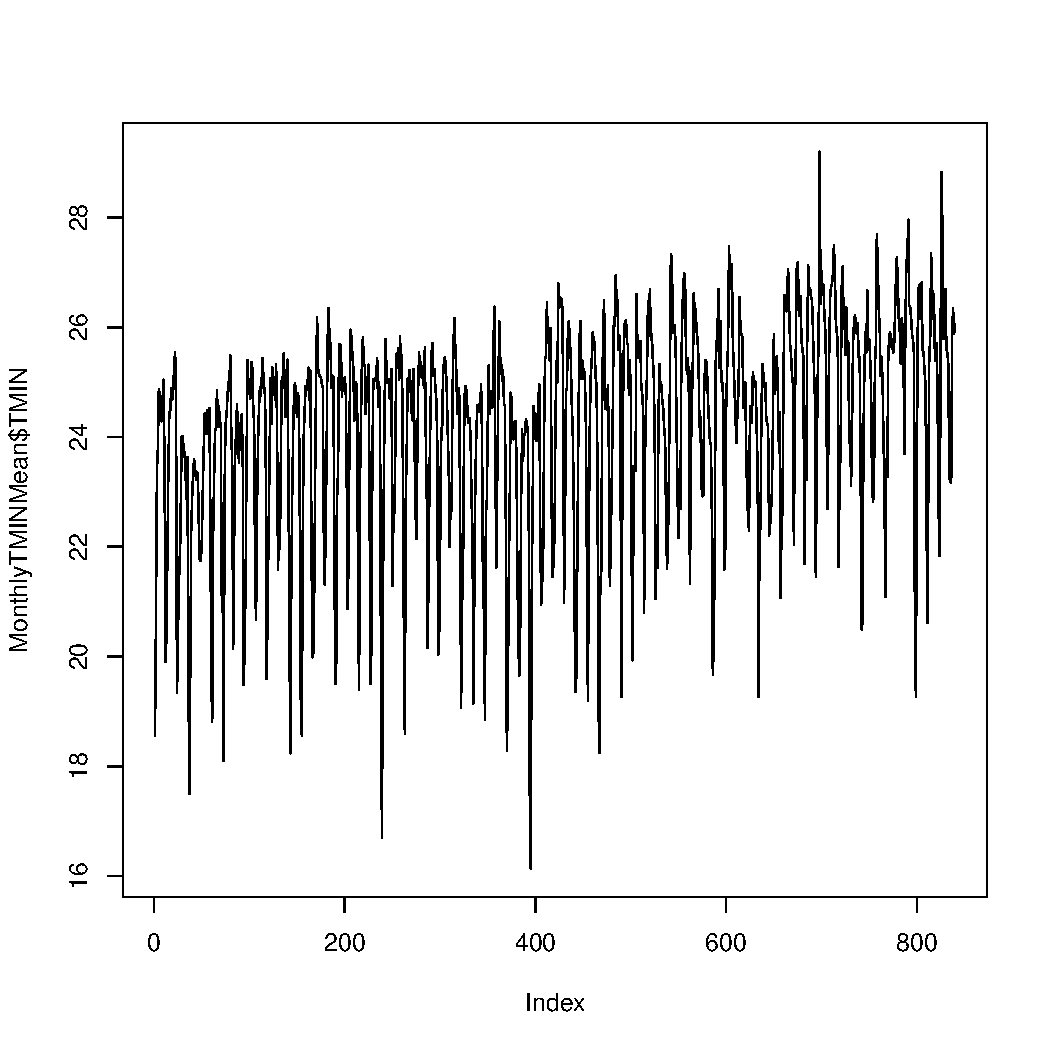
\includegraphics[width=\maxwidth]{figure/unnamed-chunk-7-1} 

\end{knitrout}

There is still lots of scatter and now we can subset our data by month. 

\item Using the example above, we'll plot all 12 months at once to look for patterns (Table \ref{fig:TMIN}).

\begin{figure}[ht]
\caption{Twelve Months of Monthly Average Daily Minimum 
Temperatures, Bangkok, Thailand}
\label{fig:TMIN}
\begin{knitrout}
\definecolor{shadecolor}{rgb}{0.969, 0.969, 0.969}\color{fgcolor}
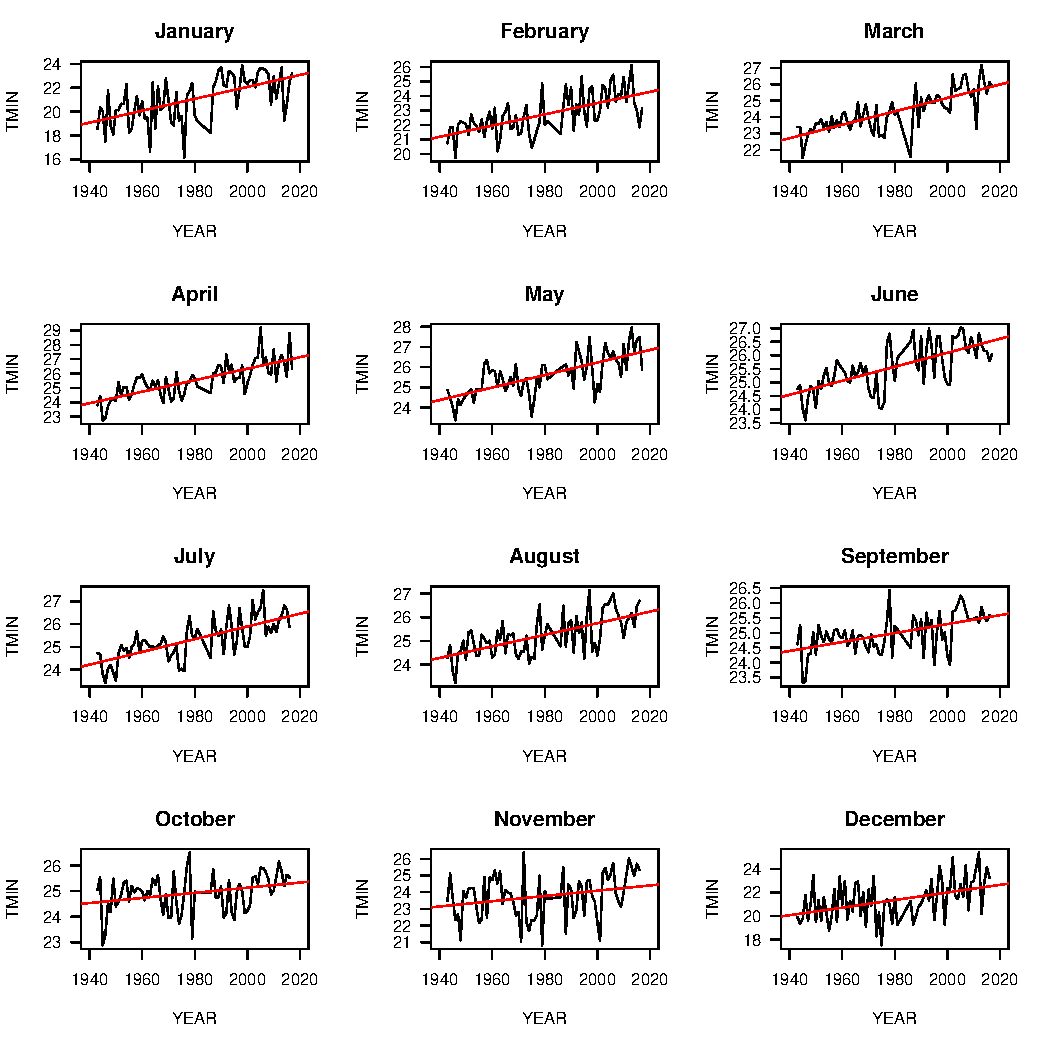
\includegraphics[width=\maxwidth]{figure/12MonthsTMIN-1} 

\end{knitrout}
\end{figure} 

\item The change in minimum temperatures seems to be even more compelling than the maximum temperatures. To compare, look at the Table \ref{tab:results} to appreciate estimated slopes and their associated null hypothesis probabilities. 

\begin{kframe}
\begin{alltt}
\hlkwd{library}\hlstd{(xtable)}
\hlstd{Results} \hlkwb{<-} \hlkwd{data.frame}\hlstd{(}\hlkwc{Month} \hlstd{= TMINresult[}\hlkwd{c}\hlstd{(}\hlnum{2}\hlopt{:}\hlnum{13}\hlstd{),}\hlnum{1}\hlstd{],} \hlkwc{TMINSlope} \hlstd{= TMINresult[}\hlkwd{c}\hlstd{(}\hlnum{2}\hlopt{:}\hlnum{13}\hlstd{),}\hlnum{2}\hlstd{],} \hlkwc{TMIN_P} \hlstd{=} \hlkwd{as.numeric}\hlstd{(TMINresult[}\hlkwd{c}\hlstd{(}\hlnum{2}\hlopt{:}\hlnum{13}\hlstd{),}\hlnum{3}\hlstd{]),} \hlkwc{TMINRsq} \hlstd{= TMINresult[}\hlkwd{c}\hlstd{(}\hlnum{2}\hlopt{:}\hlnum{13}\hlstd{),}\hlnum{4}\hlstd{],} \hlkwc{TMAXSlope} \hlstd{= TMAXresult[}\hlkwd{c}\hlstd{(}\hlnum{2}\hlopt{:}\hlnum{13}\hlstd{),}\hlnum{2}\hlstd{],} \hlkwc{TMAX_P} \hlstd{=} \hlkwd{as.numeric}\hlstd{(TMAXresult[}\hlkwd{c}\hlstd{(}\hlnum{2}\hlopt{:}\hlnum{13}\hlstd{),}\hlnum{3}\hlstd{]),} \hlkwc{TMAXRsq} \hlstd{= TMAXresult[}\hlkwd{c}\hlstd{(}\hlnum{2}\hlopt{:}\hlnum{13}\hlstd{),}\hlnum{4}\hlstd{])}
\hlstd{Results}\hlopt{$}\hlstd{starTMIN} \hlkwb{=} \hlstr{"NS"}
\hlstd{Results}\hlopt{$}\hlstd{starTMIN[Results}\hlopt{$}\hlstd{TMIN_P} \hlopt{<=} \hlnum{.05}\hlstd{]} \hlkwb{=} \hlstr{"*"}
\hlstd{Results}\hlopt{$}\hlstd{starTMIN[Results}\hlopt{$}\hlstd{TMIN_P} \hlopt{<} \hlnum{0.01}\hlstd{]} \hlkwb{=} \hlstr{"**"}
\hlstd{Results}\hlopt{$}\hlstd{starTMIN[Results}\hlopt{$}\hlstd{TMIN_P} \hlopt{<} \hlnum{0.001}\hlstd{]} \hlkwb{=} \hlstr{"***"}
\hlstd{Results}\hlopt{$}\hlstd{starTMAX} \hlkwb{=} \hlstr{"NS"}
\hlstd{Results}\hlopt{$}\hlstd{starTMAX[Results}\hlopt{$}\hlstd{TMAX_P} \hlopt{<} \hlnum{0.05}\hlstd{]} \hlkwb{=} \hlstr{"*"}
\hlstd{Results}\hlopt{$}\hlstd{starTMAX[Results}\hlopt{$}\hlstd{TMAX_P} \hlopt{<} \hlnum{0.01}\hlstd{]} \hlkwb{=} \hlstr{"**"}
\hlstd{Results}\hlopt{$}\hlstd{starTMAX[Results}\hlopt{$}\hlstd{TMAX_P} \hlopt{<} \hlnum{0.001}\hlstd{]} \hlkwb{=} \hlstr{"***"}
\hlstd{Results}\hlopt{$}\hlstd{TMINslope}\hlkwb{=}\hlkwd{paste}\hlstd{(Results}\hlopt{$}\hlstd{TMINSlope, Results}\hlopt{$}\hlstd{starTMIN)}
\hlstd{Results}\hlopt{$}\hlstd{TMAXslope}\hlkwb{=}\hlkwd{paste}\hlstd{(Results}\hlopt{$}\hlstd{TMAXSlope, Results}\hlopt{$}\hlstd{starTMAX)}
\hlkwd{colnames}\hlstd{(Results)} \hlkwb{<-} \hlkwd{c}\hlstd{(}\hlstr{"Month"}\hlstd{,} \hlstr{"2"}\hlstd{,} \hlstr{"3"}\hlstd{,} \hlstr{"R^2"}\hlstd{,} \hlstr{"5"}\hlstd{,} \hlstr{"6"}\hlstd{,}
                       \hlstr{"R^2"}\hlstd{,} \hlstr{"8"}\hlstd{,} \hlstr{"9"}\hlstd{,} \hlstr{"Slope TMIN"}\hlstd{,} \hlstr{"Slope TMAX"}\hlstd{)}
\hlkwd{print}\hlstd{(}\hlkwd{xtable}\hlstd{(Results[,}\hlkwd{c}\hlstd{(}\hlnum{1}\hlstd{,} \hlnum{10}\hlstd{,} \hlnum{4}\hlstd{,} \hlnum{11}\hlstd{,} \hlnum{7}\hlstd{)]))}
\end{alltt}
\end{kframe}% latex table generated in R 3.4.1 by xtable 1.8-2 package
% Fri Sep  7 11:47:21 2018
\begin{table}[ht]
\centering
\begin{tabular}{rlllll}
  \hline
 & Month & Slope TMIN & R\verb|^|2 & Slope TMAX & R\verb|^|2.1 \\ 
  \hline
1 & January & 0.0498 *** & 0.341 & -0.0051 NS & 0.009 \\ 
  2 & February & 0.0387 *** & 0.385 & -1e-04 NS & 0 \\ 
  3 & March & 0.0409 *** & 0.567 & -0.002 NS & 0.001 \\ 
  4 & April & 0.04 *** & 0.551 & 0.0097 NS & 0.035 \\ 
  5 & May & 0.031 *** & 0.48 & 0.0088 NS & 0.021 \\ 
  6 & June & 0.0259 *** & 0.448 & 0.0129 * & 0.078 \\ 
  7 & July & 0.028 *** & 0.493 & 0.0157 *** & 0.173 \\ 
  8 & August & 0.0245 *** & 0.395 & 0.0194 *** & 0.245 \\ 
  9 & September & 0.015 *** & 0.279 & 0.0217 *** & 0.257 \\ 
  10 & October & 0.01 * & 0.093 & 0.02 *** & 0.174 \\ 
  11 & November & 0.0158 * & 0.067 & 0.0253 *** & 0.169 \\ 
  12 & December & 0.0322 *** & 0.178 & 0.0119 NS & 0.034 \\ 
   \hline
\end{tabular}
\end{table}


Based on the results above, the slopes are greatest during the dry season (starting in May) for the maximum temperatures -- but the minimum temperatures show the largest slopes (change) and peaking between January and April.  

In addition, the $r^2$ values signify the amount of the variance explained by the predictor -- in the case of TMIN, most of the values are over 20\% meaning that over 20\% of the variance is explained by time. While in March and April over time explains 50\% of the variance. 

This is very high for uncontrolled experiments. However, we should be cognizant that in many cases, especially for the maximum temperatures, it is less than 10\%. This means the the variation in temperature are not predicted by time -- thus, as a modeler, I would work very hard to capture other sources to better understand what is going on in Thailand. 

Finally, we should also be very concerned about testing 2 dozen hypotheses with our little R code. It's easy to do, but based on change alone, with a critical value of 0.05, we should expect 1 in 20 tests to give us a Type I error, a signal when one doesn't exists. Since we did 12 tests, we should expect a good chance that one or more of our tests will reject the null hypothesis incorrectly. Yikes!  
Please keep this in mind and be careful to avoid this potential problem. 

As we might expect, the a small amount of the variance is explained by the ``Month.'' Many things predict temerpature, that year is one, is quite problematic.

\item What we have not determined is the cause. So, be careful when you describe the results, cause and effect cannot be analyzed using this method.

\end{enumerate}

\subsubsection{Precipitation: Departure from Mean}

Precipiation might depend more on the departure from the mean (often referred as as normal, whatever that means!).  I think it's worth pursuing, but haven't finished the analysis yet.

Precipitation is something that might increase or decrease due to climate change. So, to analyze this, we will evaluate how much precipitation has deveated from the mean, by plotting the rainfall and the mean in a time-series plot. 

Second, we need to remove the missing values and evalaute which years have complete years. If you are missing rainy months, then the whole year should be thrown out -- but what about partial years in the drought season? We'll need to be consistent -- assuming that missing data are not zeros, we'll define complete years as over 300 days of data. 

NOTE: The missing values have not been converted to NAs!
\begin{knitrout}
\definecolor{shadecolor}{rgb}{0.969, 0.969, 0.969}\color{fgcolor}\begin{kframe}
\begin{alltt}
\hlstd{climate_data}\hlopt{$}\hlstd{PRCP[climate_data}\hlopt{$}\hlstd{PRCP}\hlopt{==-}\hlnum{9999}\hlstd{]} \hlkwb{<-} \hlnum{NA}

\hlstd{Missing} \hlkwb{<-} \hlkwd{aggregate}\hlstd{(}\hlkwd{is.na}\hlstd{(climate_data}\hlopt{$}\hlstd{PRCP),}
          \hlkwd{list}\hlstd{(climate_data}\hlopt{$}\hlstd{Month, climate_data}\hlopt{$}\hlstd{Year), sum)}

\hlcom{# The aggregate command is used to create a simplified dataset. In this case}
\hlcom{# we are creating a sum of PRCP based on each month and year.}

\hlstd{Missing}\hlopt{$}\hlstd{Date} \hlkwb{=} \hlkwd{as.numeric}\hlstd{(Missing}\hlopt{$}\hlstd{Group.1)} \hlopt{+} \hlkwd{as.numeric}\hlstd{(Missing}\hlopt{$}\hlstd{Group.2)}\hlopt{/}\hlnum{12}

\hlkwd{plot}\hlstd{(x} \hlopt{~} \hlstd{Date,} \hlkwc{data}\hlstd{=Missing)}
\end{alltt}
\end{kframe}
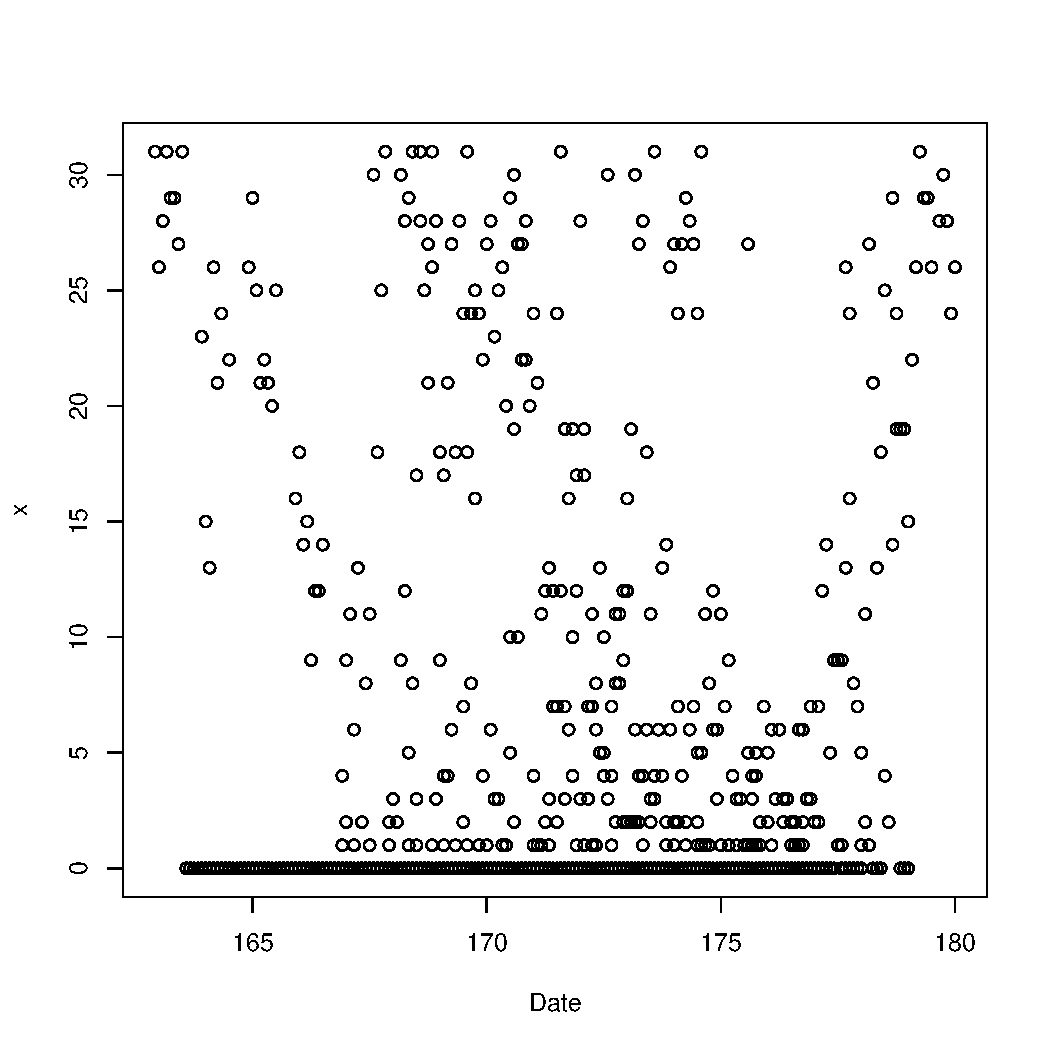
\includegraphics[width=\maxwidth]{figure/unnamed-chunk-9-1} 

\end{knitrout}

Third, we will need to decide what level of aggredation -- monthly, yearly, etc.  Let's aggreate by month and year to get monthly totals. 

There are loads of missing values in many months. Let's cut of the months that have more than 4 missing days. 

\begin{knitrout}
\definecolor{shadecolor}{rgb}{0.969, 0.969, 0.969}\color{fgcolor}\begin{kframe}
\begin{alltt}
\hlstd{TotalPPT} \hlkwb{<-} \hlkwd{aggregate}\hlstd{(climate_data}\hlopt{$}\hlstd{PRCP,}
            \hlkwd{list}\hlstd{(climate_data}\hlopt{$}\hlstd{Month, climate_data}\hlopt{$}\hlstd{Year), sum,} \hlkwc{na.rm}\hlstd{=T)}

\hlcom{# Check to see what you created.}

\hlkwd{names}\hlstd{(TotalPPT)} \hlkwb{=} \hlkwd{c}\hlstd{(}\hlstr{"Group.1"}\hlstd{,} \hlstr{"Group.2"}\hlstd{,} \hlstr{"ppt"}\hlstd{)}

\hlstd{NonMissing} \hlkwb{<-} \hlstd{Missing[Missing}\hlopt{$}\hlstd{x} \hlopt{<} \hlnum{5}\hlstd{,} \hlkwd{c}\hlstd{(}\hlnum{1}\hlopt{:}\hlnum{3}\hlstd{)]}
\hlkwd{library}\hlstd{(dplyr)}
\end{alltt}


{\ttfamily\noindent\itshape\color{messagecolor}{\#\# \\\#\# Attaching package: 'dplyr'}}

{\ttfamily\noindent\itshape\color{messagecolor}{\#\# The following objects are masked from 'package:stats':\\\#\# \\\#\#\ \ \ \  filter, lag}}

{\ttfamily\noindent\itshape\color{messagecolor}{\#\# The following objects are masked from 'package:base':\\\#\# \\\#\#\ \ \ \  intersect, setdiff, setequal, union}}\begin{alltt}
\hlstd{PPT} \hlkwb{<-} \hlkwd{merge}\hlstd{(TotalPPT, NonMissing,} \hlkwc{all.y}\hlstd{=}\hlnum{TRUE}\hlstd{)}
\hlstd{PPT}\hlopt{$}\hlstd{Date} \hlkwb{<-} \hlkwd{as.numeric}\hlstd{(PPT}\hlopt{$}\hlstd{Group.1)} \hlopt{+} \hlkwd{as.numeric}\hlstd{(PPT}\hlopt{$}\hlstd{Group.2)}\hlopt{/}\hlnum{12}
\hlkwd{head}\hlstd{(PPT)}
\end{alltt}
\begin{verbatim}
##   Group.1 Group.2  ppt x     Date
## 1      01    1951  0.2 0 163.5833
## 2      01    1952  0.0 0 163.6667
## 3      01    1953 20.3 0 163.7500
## 4      01    1954  5.3 0 163.8333
## 5      01    1955  2.2 0 163.9167
## 6      01    1956  5.6 0 164.0000
\end{verbatim}
\end{kframe}
\end{knitrout}

First, we need a "mean" -- The IPCC uses 1961-1990 as a norm for temperature, I don't know what is the standard for rainfall or Thailand, so we should look that up. For now, we'll use our filtered records to generate a mean.

\begin{knitrout}
\definecolor{shadecolor}{rgb}{0.969, 0.969, 0.969}\color{fgcolor}\begin{kframe}
\begin{alltt}
\hlstd{PRCP_mean} \hlkwb{=} \hlkwd{mean}\hlstd{(PPT}\hlopt{$}\hlstd{ppt)}
\end{alltt}
\end{kframe}
\end{knitrout}

\begin{knitrout}
\definecolor{shadecolor}{rgb}{0.969, 0.969, 0.969}\color{fgcolor}\begin{kframe}
\begin{alltt}
\hlkwd{plot}\hlstd{(ppt}\hlopt{~}\hlstd{Date,} \hlkwc{data}\hlstd{=PPT)}
\hlkwd{abline}\hlstd{(}\hlkwc{h}\hlstd{=PRCP_mean,} \hlkwc{col}\hlstd{=}\hlstr{"blue"}\hlstd{)}
\end{alltt}
\end{kframe}
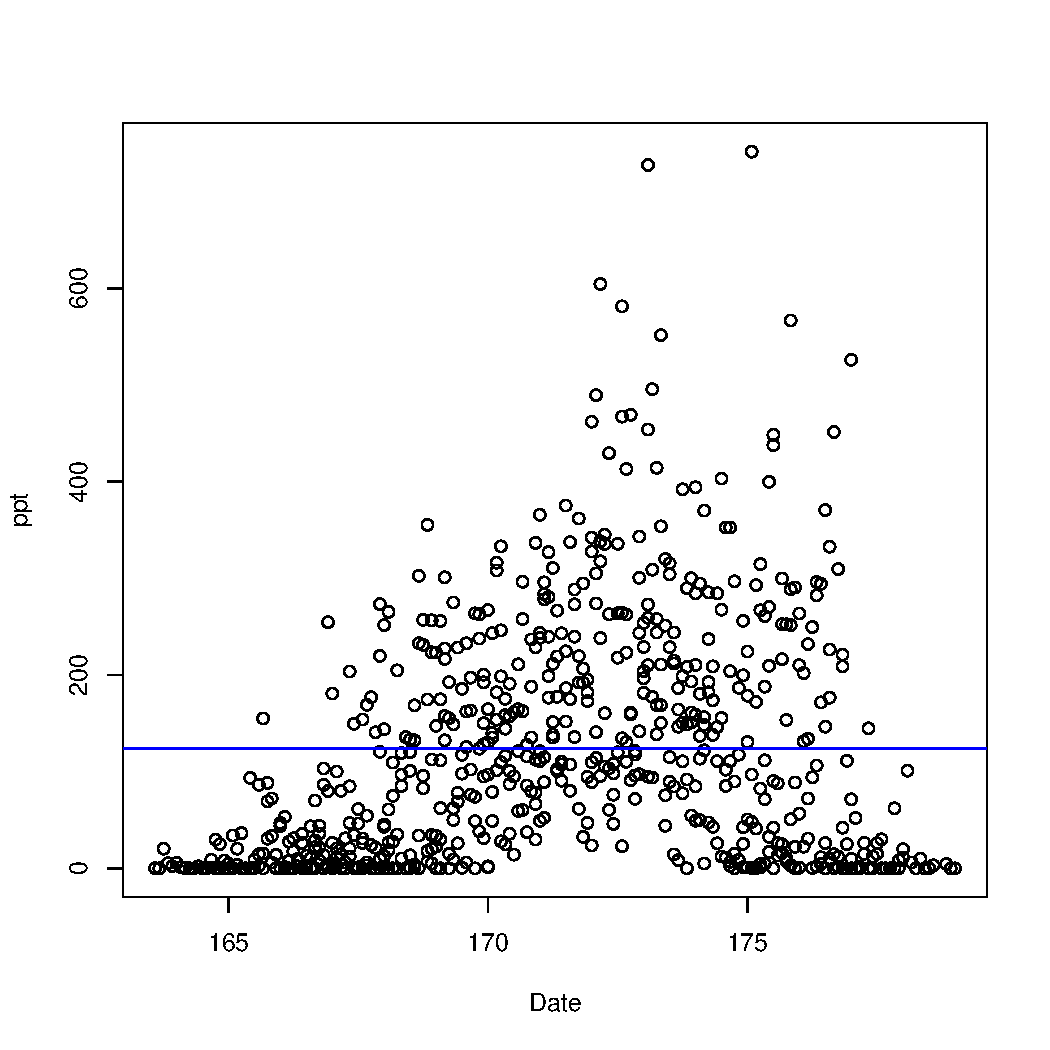
\includegraphics[width=\maxwidth]{figure/unnamed-chunk-12-1} 

\end{knitrout}

Wow, these data look terrible -- the mean looks meaningless given the biased data set. I don't think we can do more analysis with this. But let's look at a few months and see what we can decipher.

\begin{figure}
\begin{knitrout}
\definecolor{shadecolor}{rgb}{0.969, 0.969, 0.969}\color{fgcolor}
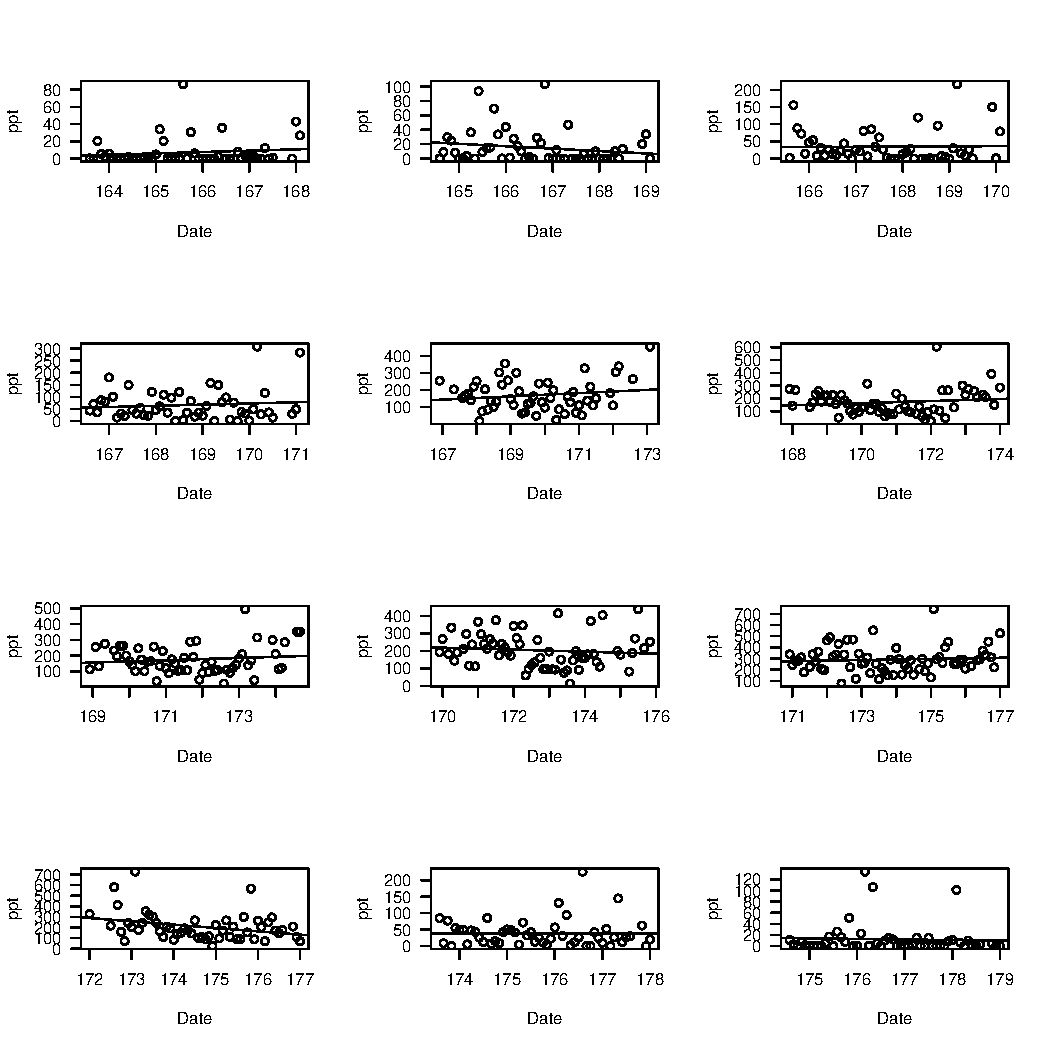
\includegraphics[width=\maxwidth]{figure/unnamed-chunk-13-1} 

\end{knitrout}
\end{figure}
 
%Fourth, in CA the water year starts in Oct 1. Should we follow the same convention?

\begin{knitrout}
\definecolor{shadecolor}{rgb}{0.969, 0.969, 0.969}\color{fgcolor}\begin{kframe}
\begin{alltt}
\hlcom{#LosAngeles$PRCP[LosAngeles$PRCP==-9999] <- NA}
\hlcom{#YearlySum = aggregate(PRCP ~ Year, LosAngeles, sum)}
\hlcom{#YearlySum$YEAR = as.numeric(YearlySum$Year) }
\hlcom{#YearlyMean = mean(YearlySum$PRCP)}
\end{alltt}
\end{kframe}
\end{knitrout}

A yearly mean, based on the annual sum for the entire records. Not sure this is appropriate.

Figure has points of the yearly sum of rainfall and the blue line mean. The greenline is the trend and red line is a five year running average, I think!  I am still trying to understand what the code is doing.

\begin{knitrout}
\definecolor{shadecolor}{rgb}{0.969, 0.969, 0.969}\color{fgcolor}\begin{kframe}
\begin{alltt}
\hlcom{#plot(PRCP~YEAR, data=YearlySum, las=1, ty="p")}
\hlcom{#abline(h=YearlyMean, col="blue")}
\hlcom{#YearlySum.lm = lm(PRCP~YEAR, data=YearlySum)}
\hlcom{#abline(coef(YearlySum.lm), col="green")}

\hlcom{#n <- 5}
\hlcom{#k <- rep(1/n, n)}
\hlcom{#k}

\hlcom{#y_lag <- stats::filter(YearlySum$PRCP, k, sides=1)}
\hlcom{#lines(YearlySum$YEAR, y_lag, col="red")}
\end{alltt}
\end{kframe}
\end{knitrout}

%The model suggests that the precipitation is declining at a rate of `r coef(YearlySum.lm)[2]` cm yr$^{-1}~$, or `r round(coef(YearlySum.lm)[2]*10, 2)` cm decade$^{-1}$.

\begin{knitrout}
\definecolor{shadecolor}{rgb}{0.969, 0.969, 0.969}\color{fgcolor}\begin{kframe}
\begin{alltt}
\hlcom{#summary(YearlySum.lm)}
\end{alltt}
\end{kframe}
\end{knitrout}

\subsection{Assumptions of the Linear Regression}

Regression models, like all statistics, rely on certain assumptions. Violations of these assumptions reduces the validity of the model. If the violations are serious, then the model could be misleading or even incorrect.

TBD

%Here is a list of assumptions to produce a valid regression model:

%\begin{description}
%  \item[Homogeneity of Variance]
%  \item[something else]
%\end{description}

\subsubsection{Assumptions about $\epsilon$}

The error term should have 


\begin{description}
  \item [E(et) = 0], zero mean

  \item[E(et) = s], constant variance

  \item[E(et, Xt) = 0] , no correlation with X 

  \item[TBD] E(e , e ), no autocorrelation. t t-1

  \item[e ~ Normally distributed] (for hypothesis testing). 

\end{description}

Assumption four is especially important and most likely not to be met when using time series data.

Autocorrelation.

1. It is not uncommon for errors to “track’ themselves; that is, for the error a time t to depend in part on its value at t - m, where m is a prior time period.

\subsubsection{Model Diagnostics}

With every statistical test done, researchers validate their model in some way or anther. Often this entails the use of diagnostics, a standardize battery of procedures to check to see if the data are following the assumptions. 

In R four plots are created by default.  To see them all at the same time, we need to change the graphical parameters, using the par() function. In this case, we use \texttt{par(mfrow=c(2,2))} to create alter the graphics window expects four panels, in this case a 2 rows and two columns.

Try not to get bogged down in the code at this point. But noting this function can be handy in a number of ways to improve one's graphics. 

% Additional LaTeX code to add caption to figure
\begin{figure}
\label{fig:diagnostics}
\caption{Default diagnostic plots for a linear model in R.}
%\setkeys{Gin}{width=0.75\textwidth} % LaTeX code to read the graphic file in at 75% of its original size
% R code chunk that produces a graphic
\begin{knitrout}
\definecolor{shadecolor}{rgb}{0.969, 0.969, 0.969}\color{fgcolor}\begin{kframe}
\begin{alltt}
\hlkwd{par}\hlstd{(}\hlkwc{mfrow}\hlstd{=}\hlkwd{c}\hlstd{(}\hlnum{2}\hlstd{,}\hlnum{2}\hlstd{))}
\hlkwd{plot}\hlstd{(}\hlkwd{lm}\hlstd{(TMIN} \hlopt{~} \hlstd{YEAR,} \hlkwc{data}\hlstd{=MonthlyTMINMean[MonthlyTMINMean}\hlopt{$}\hlstd{MONTH}\hlopt{==}\hlnum{1}\hlstd{,]))}
\end{alltt}
\end{kframe}
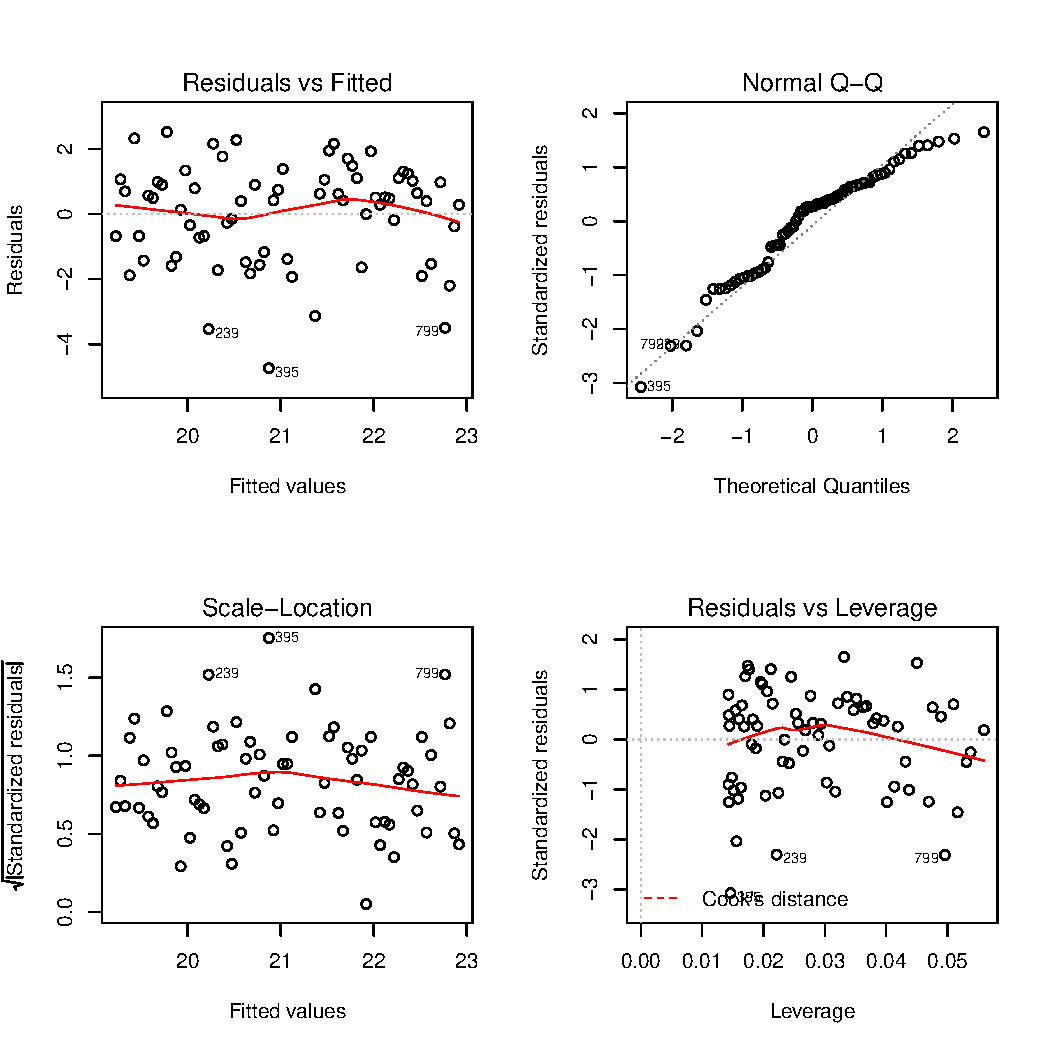
\includegraphics[width=\maxwidth]{figure/unnamed-chunk-17-1} 

\end{knitrout}
\end{figure}

To determine the validity of linear model assumptions (e.g. normality or heterogeneity of variance), you have probably used statistical tests; in contrast statisticians almost exclusively look at diagnostic plots. Why?  When assumptions are violated the tests to determine violations do not perform well. So, let's see how to look at these assumptions graphically with these diagnostic plots. Linear models should have diagnostic plots that do not have any obvious structure or pattern. In this case, Figure~\ref{fig:diagnostics} should show a great deal remaining structure in the residuals. Although for today, we are not going to try to interpret these figures, but you should notice there is a ton of unaccounted structure, i.e. variance, in the model. This is due, in part, to a violation of independence; these data are serially correlated and the model does not account for that and is inappropriate because of this. It also appears that a straight-line model does not fit well and a curvilinear should be investigated.

A properly specified model is shown in 

%Figure~\ref{fig:co2_data_mlo}. In this case, the trend line has been developing using a time series analysis, which is beyond the scope of this course. Nevertheless, you want to keep this in mind during the semester because we will see a fair amount of data that looks like this.

\end{document}
